% 04-Marco_Teorico_Presentacion_Tesis.tex
% Diapositivas de la sección Marco Teórico

\section{Marco Teórico}

\begin{frame}
\frametitle{Redes Neuronales Convolucionales (CNN)}
\begin{itemize}
    \item Las CNN son la base del análisis de imágenes médicas.
    \item Permiten extraer características espaciales relevantes de las imágenes.
    \item Se utilizan ampliamente en tareas de clasificación, segmentación y detección.
\end{itemize}
\begin{figure}[ht!]
    \centering
    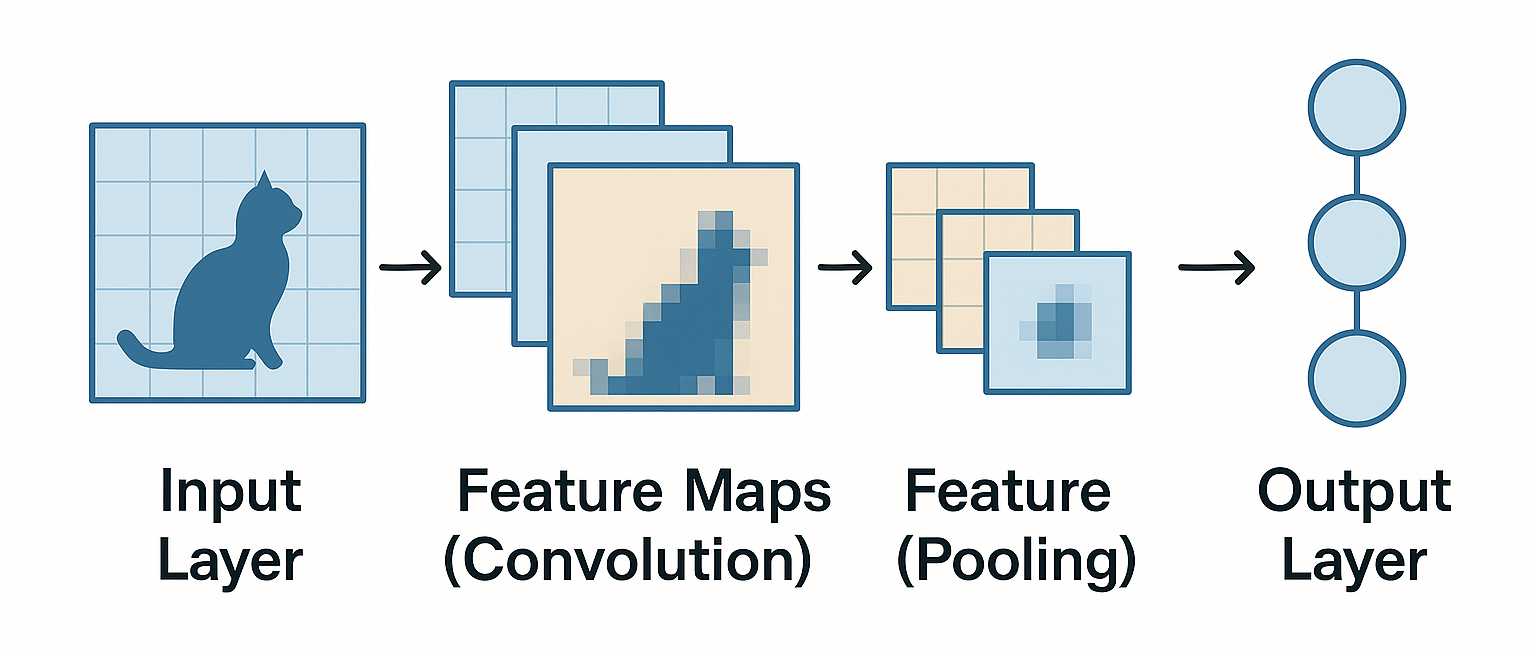
\includegraphics[width=0.5\textwidth]{images/convolutional_network.png}
    \caption{Esquema de referencia de una red neuronal convolucional.}
\end{figure}
\end{frame}

\begin{frame}
\frametitle{Estructura de una red convolucional}
\begin{itemize}
    \item \textbf{Capa de Convolución}: Extrae características locales (bordes, texturas, patrones) mediante filtros (kernels).
    \item \textbf{Capa de Activación} (ReLU, LeakyReLU, etc.): Introduce no linealidad y elimina valores negativos.
    \item \textbf{Capa de Pooling}: Reduce la dimensionalidad conservando la información más relevante.
    \item \textbf{Capas Fully Connected} (Dense): Al final de la red, se aplanan los feature maps y se conectan a neuronas tradicionales para clasificación/regresión.
\end{itemize}
\end{frame}

\begin{frame}
\frametitle{Aplicaciones de una red convolucional}
\begin{itemize}
    \item \textbf{Clasificación de imágenes}: ResNet, VGG
    \item \textbf{Detección de objetos}: YOLO, Faster R-CNN
    \item \textbf{Segmentación semántica}: U-Net
    \item \textbf{Procesamiento de lenguaje natural}: CNNs para texto
\end{itemize}
\begin{figure}[ht!]
    \centering
    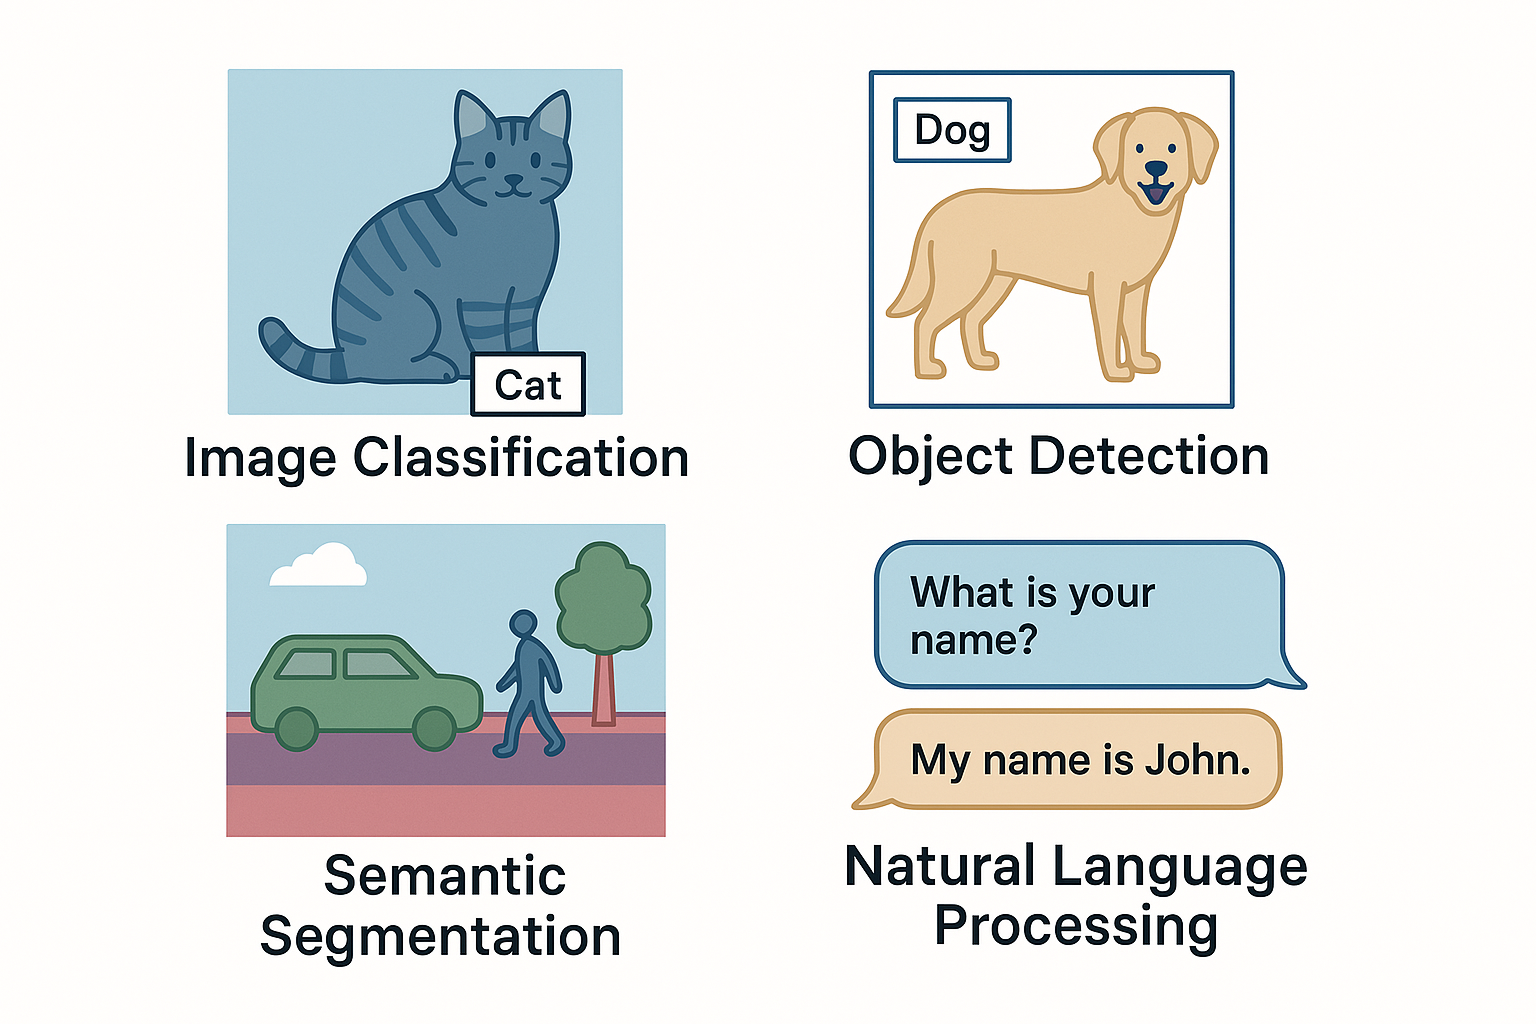
\includegraphics[width=0.4\textwidth]{images/cnn_applications.png}
    \caption{Aplicaciones de una red neuronal convolucional.}
\end{figure}
\end{frame}

\begin{frame}
\frametitle{ResNet50: Arquitectura Residual}
\begin{itemize}
    \item ResNet50 es una arquitectura profunda con 50 capas y conexiones residuales.
    \item Facilita el entrenamiento de redes muy profundas evitando el problema del desvanecimiento del gradiente.
    \item En esta tesis, ResNet50 se emplea como backbone para la extracción de características en imágenes de rayos X.
\end{itemize}
\begin{figure}[ht!]
    \centering
    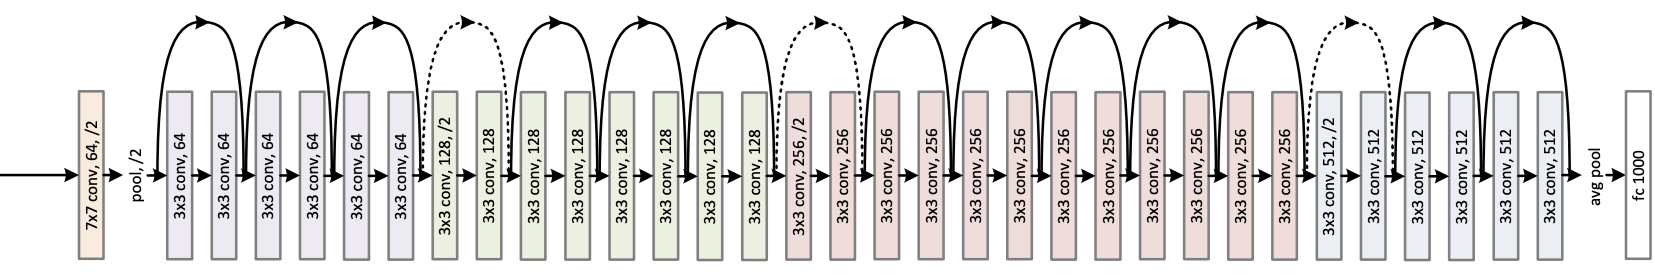
\includegraphics[width=0.8\textwidth]{images/resnet50_architecture.png}
    \caption{Arquitectura base de un modelo ResNet.}
\end{figure}
\end{frame}

\begin{frame}
\frametitle{¿Por qué ResNet50 para esta tesis?}
\begin{itemize}
    \item \textbf{Buen rendimiento}: Probado en tareas de clasificación de imágenes médicas
    \item \textbf{Arquitectura establecida}: Ampliamente validada en la comunidad científica
    \item \textbf{Balance óptimo}: Entre profundidad y eficiencia computacional
    \item \textbf{Transfer learning efectivo}: Desde ImageNet a imágenes médicas
    \item \textbf{Capacidad de captura}: Características complejas en imágenes de rayos X
\end{itemize}
\end{frame}

\begin{frame}
\frametitle{Redes Neuronales Recurrentes (RNN)}
\begin{itemize}
    \item Las RNN procesan secuencias de datos, manteniendo información temporal.
    \item Son útiles para tareas donde el contexto previo es importante.
    \item Existen variantes como LSTM y GRU que mejoran la capacidad de memoria.
\end{itemize}
\begin{figure}[ht!]
    \centering
    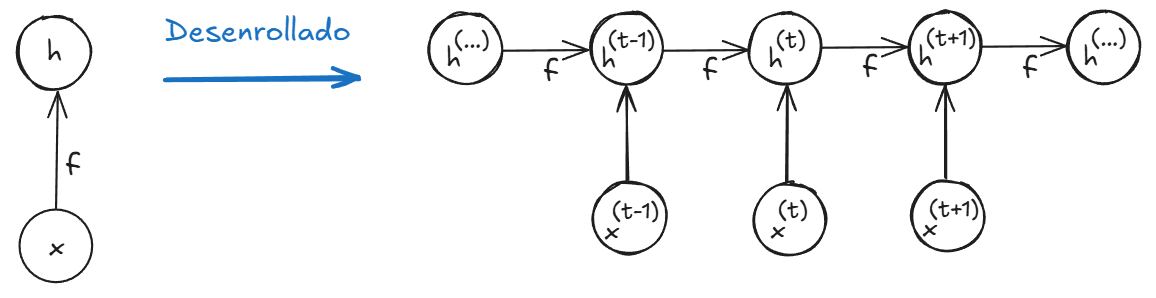
\includegraphics[width=0.7\textwidth]{../Chapters/2. Transformer/Figures/rnn/rnn_cgraph.png}
    \caption{Grafo computacional de una RNN desenrollada.}
\end{figure}
\end{frame}

\begin{frame}
\frametitle{Mecanismos de Atención y Transformers}
\begin{itemize}
    \item Los mecanismos de atención permiten al modelo enfocarse en partes relevantes de la entrada.
    \item Los Transformers revolucionaron el procesamiento de secuencias al permitir el procesamiento paralelo y el uso de atención múltiple (Multi-Head Attention).
    \item Vision Transformer (ViT) aplica estos conceptos a imágenes.
\end{itemize}
\end{frame}

\begin{frame}
\frametitle{Resumen del Marco Teórico}
\begin{itemize}
    \item Se combinan arquitecturas convolucionales (ResNet50) y modelos basados en atención (Transformers) para la detección de patologías pulmonares.
    \item El uso de Transfer Learning y Fine-Tuning permite adaptar modelos preentrenados a imágenes médicas.
    \item Estas técnicas mejoran la precisión y la interpretabilidad en el diagnóstico asistido por IA.
\end{itemize}
\end{frame}
